% Jet sketches for Chapter II (fig:jets_sketch), in the style of I. Neutelings' TikZ figures.
% Adapted from https://tikz.net/jet_btag/ and https://tikz.net/jet_top/ (Izaak Neutelings, CC BY-SA 4.0).
% Each tikzpicture is one page of the PDF: page 1 is panel (a), page 2 is panel (b).
\documentclass[tikz,border=2pt]{standalone}
\usepackage[T1]{fontenc}
\usepackage{cochineal}
\usepackage[cochineal]{newtxmath}
\usepackage{tikz}
\usepackage[outline]{contour} % glow around text
\usetikzlibrary{calc,math,arrows.meta}
\contourlength{0.6pt}
\tikzset{>=latex}

\colorlet{myred}{red!80!black}
\colorlet{myblue}{blue!75!black}
\colorlet{mygreen}{green!45!black}
\colorlet{mylightgreen}{green!70!black}
\colorlet{myorange}{orange!80!red!85!black}
\colorlet{myviolet}{blue!60!red!55!white}
\tikzstyle{track}=[->,line width=0.6,opacity=0.4,blue!40!black]
\tikzstyle{beam}=[myorange!35,dashed,line width=0.7,line cap=round]
\tikzstyle{mydashed}=[dash pattern=on 2pt off 2.5pt,line cap=round]
\tikzstyle{myshortdashed}=[dash pattern=on 1.5pt off 2pt,line cap=round]
\tikzstyle{measure}=[{Latex[length=2.2,width=2.2]}-{Latex[length=2.2,width=2.2]}]

% \jetcone[color]{apex}{centre of base}{opening angle}{eccentricity of base}{extra drawing}
% The extra drawing is placed between the base and the translucent front of the cone,
% in a scope rotated along the jet axis, where \a and \b are the radii of the base.
\newcommand\jetcone[6][blue]{{
  \pgfmathanglebetweenpoints{\pgfpointanchor{#2}{center}}{\pgfpointanchor{#3}{center}}
  \edef\ang{#4/2}
  \edef\e{#5}
  \edef\vang{\pgfmathresult}
  \tikzmath{
    coordinate \C;
    \C = (#2)-(#3);
    \x = veclen(\Cx,\Cy)*\e*sin(\ang)^2;
    \y = tan(\ang)*(veclen(\Cx,\Cy)-\x);
    \a = veclen(\Cx,\Cy)*sqrt(\e)*sin(\ang);
    \b = veclen(\Cx,\Cy)*tan(\ang)*sqrt(1-\e*sin(\ang)^2);
    \angb = acos(sqrt(\e)*sin(\ang));
  }
  \coordinate (tmpL) at ($(#3)-(\vang:\x pt)+(\vang+90:\y pt)$);
  \coordinate (tmpO) at ($(#2)+(\vang:0.01)$);
  \coordinate (tmpO') at ($(#2)+(\vang:0.02)$);
  \fill[white,rotate=\vang]
    (tmpL) arc(180-\angb:180+\angb:{\a pt} and {\b pt}) -- (tmpO) -- cycle;
  \draw[thin,#1!40!black,rotate=\vang,
    top color=#1!45!black!60,bottom color=#1!60!black!50,shading angle=\vang]
    (#3) ellipse({\a pt} and {\b pt});
  \begin{scope}[rotate=\vang]
    #6
  \end{scope}
  \draw[thin,#1!30!black,rotate=\vang,
    top color=#1!90!black!80,bottom color=#1!25!black!90,shading angle=\vang,fill opacity=0.3]
    (tmpL) arc(180-\angb:180+\angb:{\a pt} and {\b pt}) -- (tmpO) -- cycle;
}}

\newcommand\rightAngle[4]{
  \pgfmathanglebetweenpoints{\pgfpointanchor{#2}{center}}{\pgfpointanchor{#1}{center}}
  \pgfmathsetmacro\tmpx{\pgfmathresult}
  \pgfmathanglebetweenpoints{\pgfpointanchor{#2}{center}}{\pgfpointanchor{#3}{center}}
  \pgfmathsetmacro\tmpy{\pgfmathresult}
  \draw[green!20!black] (#2)++(\tmpx:#4) --++ (\tmpy:#4) --++ (\tmpx+180:#4);
}

\begin{document}

% (a) b JET WITH A DISPLACED SECONDARY VERTEX
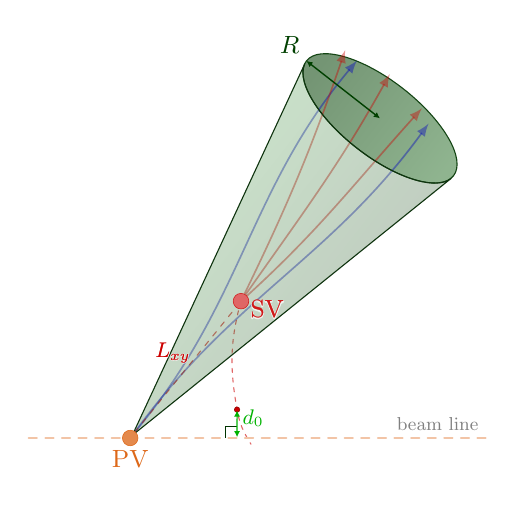
\begin{tikzpicture}[scale=4.3,baseline=(O),every node/.style={font=\small}]
  \def\R{1.0}
  \coordinate (O) at (0,0);
  \coordinate (BJ) at (52:1.20*\R);
  \coordinate (SV) at (51:0.52*\R);
  \draw[beam] (-0.30,0) -- (0,0);
  \jetcone[green!60!black!80!white]{O}{BJ}{26}{0.17}{
    \draw[track,myblue] (tmpO') to[out=-2,in=178] (7:1.30*\R);
    \draw[track,myblue] (tmpO') to[out=2,in=-178] (-5.5:1.28*\R);
    \draw[track,myred] (SV) to[out=12,in=-161] (9:1.31*\R);
    \draw[track,myred] (SV) to[out=3,in=-171] (2.5:1.32*\R);
    \draw[track,myred] (SV) to[out=-10,in=176] (-3.5:1.30*\R);
    \draw[myred,myshortdashed,line width=0.4,opacity=0.6]
      (SV) to[out=-157,in=48]++ (-144:0.32*\R) coordinate(IP)
           to[out=228,in=70]++ (240:0.11*\R);
    \draw[mydashed,myred,opacity=0.6] (tmpO') -- (SV);
    \draw[measure,green!25!black,line width=0.5] (BJ) -- ++(90:\b pt) coordinate (Rtop);
  }
  \node[green!25!black,above left=-1pt] at (Rtop) {$R$};
  \path (O) -- (SV)
    node[pos=0.62,left=0,myred,scale=0.85,opacity=0.7] {\contour{white}{$L_{xy}$}}
    node[pos=0.62,left=0,myred,scale=0.85] {$L_{xy}$};
  \draw[beam] (1.05,0) -- (O);
  \node[gray,scale=0.75,above left=0] at (1.05,0) {beam line};
  % vertices
  \draw[myorange!90,fill=myorange!70,very thin] (O) circle(0.023) node[below=1] {PV};
  \draw[myred!90,fill=myred!60,very thin] (SV) circle(0.023)
    node[below=3,right=0,opacity=0.7] {\contour{white}{SV}}
    node[below=3,right=0] {SV};
  % impact parameter
  \coordinate (IPz) at (IP |- O);
  \rightAngle{O}{IPz}{IP}{0.035}
  \draw[myred!70!black,fill=myred,very thin] (IP) circle(0.008);
  \draw[mylightgreen,measure,shorten <=0.3pt,shorten >=0.3pt] (IPz) -- (IP)
    node[pos=0.7,right=-1,scale=0.85] {$d_0$};
\end{tikzpicture}

% (b) LARGE-RADIUS JET WITH TWO SUBJETS
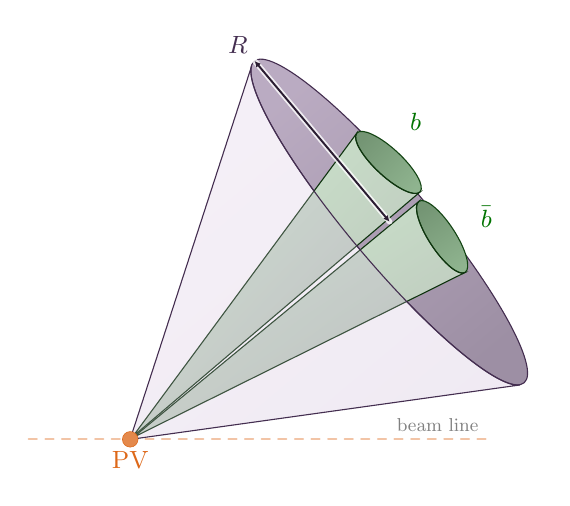
\begin{tikzpicture}[scale=4.3,baseline=(O),every node/.style={font=\small}]
  \coordinate (O) at (0,0);
  \def\vang{40}  % axis of the large jet
  \def\ang{32}   % opening angle of the large jet
  \def\e{0.05}   % eccentricity of its base
  \coordinate (BJ1) at (\vang+7:1.12);
  \coordinate (BJ2) at (\vang-7:1.10);
  \coordinate (M) at (\vang:1.00);
  \tikzmath{
    coordinate \C;
    \C = (O)-(M);
    \x = veclen(\Cx,\Cy)*\e*sin(\ang)^2;
    \y = tan(\ang)*(veclen(\Cx,\Cy)-\x);
    \a = veclen(\Cx,\Cy)*sqrt(\e)*sin(\ang);
    \b = veclen(\Cx,\Cy)*tan(\ang)*sqrt(1-\e*sin(\ang)^2);
    \angb = acos(sqrt(\e)*sin(\ang));
  }
  \coordinate (ML) at ($(M)+(\vang-180:\x pt)+(\vang+90:\y pt)$);
  \draw[beam] (-0.30,0) -- (0,0);
  % large cone, back
  \draw[thin,myviolet!40!black,rotate=\vang,
        top color=myviolet!60!black!45,bottom color=myviolet!45!black!55,shading angle=\vang]
    (M) ellipse({\a pt} and {\b pt});
  \coordinate (Rtop) at ($(M)+(\vang+90:\b pt)$);
  % subjets
  \jetcone[green!60!black!80!white]{O}{BJ1}{13}{0.10}{}
  \jetcone[green!60!black!80!white]{O}{BJ2}{13}{0.10}{}
  \node[mygreen] at (\vang+8:1.26) {$b$};
  \node[mygreen] at (\vang-8:1.24) {$\bar{b}$};
  % large cone, front
  \draw[thin,myviolet!40!black,fill opacity=0.25,rotate=\vang,rounded corners=0.001pt,
        top color=myviolet!90!black!40,bottom color=myviolet!80!black!50,shading angle=\vang]
    (ML) arc(180-\angb:180+\angb:{\a pt} and {\b pt}) -- ($(O)-(0.0005,0)$) -- cycle;
  % radius of the large jet, on top with a white halo so that it reads over the subjet
  \draw[white,line width=2.0,opacity=0.8,line cap=round] (M) -- (Rtop);
  \draw[measure,myviolet!25!black,line width=0.7] (M) -- (Rtop);
  \node[myviolet!40!black,above left=-1pt] at (Rtop) {$R$};
  \draw[beam] (1.05,0) -- (O);
  \node[gray,scale=0.75,above left=0] at (1.05,0) {beam line};
  \draw[myorange!90,fill=myorange!70,very thin] (O) circle(0.023) node[below=1] {PV};
\end{tikzpicture}

\end{document}
